\documentclass[twoside]{book}

% Packages required by doxygen
\usepackage{calc}
\usepackage{doxygen}
\usepackage{graphicx}
\usepackage[utf8]{inputenc}
\usepackage{makeidx}
\usepackage{multicol}
\usepackage{multirow}
\usepackage{textcomp}
\usepackage[table]{xcolor}

% Font selection
\usepackage[T1]{fontenc}
\usepackage{mathptmx}
\usepackage[scaled=.90]{helvet}
\usepackage{courier}
\usepackage{amssymb}
\usepackage{sectsty}
\renewcommand{\familydefault}{\sfdefault}
\allsectionsfont{%
  \fontseries{bc}\selectfont%
  \color{darkgray}%
}
\renewcommand{\DoxyLabelFont}{%
  \fontseries{bc}\selectfont%
  \color{darkgray}%
}

% Page & text layout
\usepackage{geometry}
\geometry{%
  a4paper,%
  top=2.5cm,%
  bottom=2.5cm,%
  left=2.5cm,%
  right=2.5cm%
}
\tolerance=750
\hfuzz=15pt
\hbadness=750
\setlength{\emergencystretch}{15pt}
\setlength{\parindent}{0cm}
\setlength{\parskip}{0.2cm}
\makeatletter
\renewcommand{\paragraph}{%
  \@startsection{paragraph}{4}{0ex}{-1.0ex}{1.0ex}{%
    \normalfont\normalsize\bfseries\SS@parafont%
  }%
}
\renewcommand{\subparagraph}{%
  \@startsection{subparagraph}{5}{0ex}{-1.0ex}{1.0ex}{%
    \normalfont\normalsize\bfseries\SS@subparafont%
  }%
}
\makeatother

% Headers & footers
\usepackage{fancyhdr}
\pagestyle{fancyplain}
\fancyhead[LE]{\fancyplain{}{\bfseries\thepage}}
\fancyhead[CE]{\fancyplain{}{}}
\fancyhead[RE]{\fancyplain{}{\bfseries\leftmark}}
\fancyhead[LO]{\fancyplain{}{\bfseries\rightmark}}
\fancyhead[CO]{\fancyplain{}{}}
\fancyhead[RO]{\fancyplain{}{\bfseries\thepage}}
\fancyfoot[LE]{\fancyplain{}{}}
\fancyfoot[CE]{\fancyplain{}{}}
\fancyfoot[RE]{\fancyplain{}{\bfseries\scriptsize Generated on Thu Nov 12 2015 18\-:20\-:35 for Genomic Cleres Dubois by Doxygen }}
\fancyfoot[LO]{\fancyplain{}{\bfseries\scriptsize Generated on Thu Nov 12 2015 18\-:20\-:35 for Genomic Cleres Dubois by Doxygen }}
\fancyfoot[CO]{\fancyplain{}{}}
\fancyfoot[RO]{\fancyplain{}{}}
\renewcommand{\footrulewidth}{0.4pt}
\renewcommand{\chaptermark}[1]{%
  \markboth{#1}{}%
}
\renewcommand{\sectionmark}[1]{%
  \markright{\thesection\ #1}%
}

% Indices & bibliography
\usepackage{natbib}
\usepackage[titles]{tocloft}
\setcounter{tocdepth}{3}
\setcounter{secnumdepth}{5}
\makeindex

% Hyperlinks (required, but should be loaded last)
\usepackage{ifpdf}
\ifpdf
  \usepackage[pdftex,pagebackref=true]{hyperref}
\else
  \usepackage[ps2pdf,pagebackref=true]{hyperref}
\fi
\hypersetup{%
  colorlinks=true,%
  linkcolor=blue,%
  citecolor=blue,%
  unicode%
}

% Custom commands
\newcommand{\clearemptydoublepage}{%
  \newpage{\pagestyle{empty}\cleardoublepage}%
}


%===== C O N T E N T S =====

\begin{document}

% Titlepage & ToC
\hypersetup{pageanchor=false}
\pagenumbering{roman}
\begin{titlepage}
\vspace*{7cm}
\begin{center}%
{\Large Genomic Cleres Dubois }\\
\vspace*{1cm}
{\large Generated by Doxygen 1.8.6}\\
\vspace*{0.5cm}
{\small Thu Nov 12 2015 18:20:35}\\
\end{center}
\end{titlepage}
\clearemptydoublepage
\tableofcontents
\clearemptydoublepage
\pagenumbering{arabic}
\hypersetup{pageanchor=true}

%--- Begin generated contents ---
\chapter{my first index page}
\label{index}\hypertarget{index}{}\hypertarget{index_intro_sec}{}\section{introduction}\label{index_intro_sec}
hello \hypertarget{index_install_sec}{}\section{instalation}\label{index_install_sec}
\hypertarget{index_step1}{}\subsection{Step1\-: opening the box}\label{index_step1}

\chapter{Class Index}
\section{Class List}
Here are the classes, structs, unions and interfaces with brief descriptions\-:\begin{DoxyCompactList}
\item\contentsline{section}{\hyperlink{classPool}{Pool} \\*Generator class }{\pageref{classPool}}{}
\end{DoxyCompactList}

\chapter{File Index}
\section{File List}
Here is a list of all files with brief descriptions\+:\begin{DoxyCompactList}
\item\contentsline{section}{src/\hyperlink{_fitness_constraint_t_c_l_a_p_8h}{Fitness\+Constraint\+T\+C\+L\+A\+P.\+h} \\*Constraint value greater than -\/1 }{\pageref{_fitness_constraint_t_c_l_a_p_8h}}{}
\item\contentsline{section}{src/\hyperlink{_int_constraint_t_c_l_a_p_8h}{Int\+Constraint\+T\+C\+L\+A\+P.\+h} \\*Be different then 0 }{\pageref{_int_constraint_t_c_l_a_p_8h}}{}
\item\contentsline{section}{src/\hyperlink{main_8cpp}{main.\+cpp} \\*Model Wright-\/\+Fisher, Sickle Cell Anemia, Selection \& Mutation }{\pageref{main_8cpp}}{}
\item\contentsline{section}{src/\hyperlink{main__test_8cpp}{main\+\_\+test.\+cpp} \\*Tests on the simulation of the wright fisher model }{\pageref{main__test_8cpp}}{}
\item\contentsline{section}{src/\hyperlink{_mainpage_8h}{Mainpage.\+h} }{\pageref{_mainpage_8h}}{}
\item\contentsline{section}{src/\hyperlink{_meta_pool_8cpp}{Meta\+Pool.\+cpp} \\*Description \hyperlink{class_metapool}{Metapool} }{\pageref{_meta_pool_8cpp}}{}
\item\contentsline{section}{src/\hyperlink{_meta_pool_8hpp}{Meta\+Pool.\+hpp} \\*A \hyperlink{class_pool}{Pool} of Pools }{\pageref{_meta_pool_8hpp}}{}
\item\contentsline{section}{src/\hyperlink{_meta_pool_drep_8cpp}{Meta\+Pool\+Drep.\+cpp} \\*Description \hyperlink{class_metapool_drep}{Metapool\+Drep}\+: We have chosen not to use pointers on Pools which would have alowed us to recycle the \hyperlink{class_metapool}{Metapool} class and only add a few method in \hyperlink{class_pool}{Pool}. But using pointeurs is much more expensives in terms of memory cost that we choose to do 2 different classes }{\pageref{_meta_pool_drep_8cpp}}{}
\item\contentsline{section}{src/\hyperlink{_meta_pool_drep_8hpp}{Meta\+Pool\+Drep.\+hpp} \\*A \hyperlink{class_pool}{Pool} of Drepanocitose Pools }{\pageref{_meta_pool_drep_8hpp}}{}
\item\contentsline{section}{src/\hyperlink{_pool_8cpp}{Pool.\+cpp} \\*Description pool }{\pageref{_pool_8cpp}}{}
\item\contentsline{section}{src/\hyperlink{_pool_8h}{Pool.\+h} \\*Generates a pool of alleles }{\pageref{_pool_8h}}{}
\item\contentsline{section}{src/\hyperlink{_pool_drep_8cpp}{Pool\+Drep.\+cpp} \\*Description pool c }{\pageref{_pool_drep_8cpp}}{}
\item\contentsline{section}{src/\hyperlink{_pool_drep_8h}{Pool\+Drep.\+h} \\*Generates a pool of alleles using the sickle cell anemia. This is class inherits of pool and uses the sickle cell model, based on real values }{\pageref{_pool_drep_8h}}{}
\item\contentsline{section}{src/\hyperlink{_proba_constraint_t_c_l_a_p_8h}{Proba\+Constraint\+T\+C\+L\+A\+P.\+h} \\*Constraint we want to apply to the inputs of the user }{\pageref{_proba_constraint_t_c_l_a_p_8h}}{}
\item\contentsline{section}{src/\hyperlink{_vector_constraint_t_c_l_a_p_8h}{Vector\+Constraint\+T\+C\+L\+A\+P.\+h} \\*Constraint we want to apply to the inputs of the user }{\pageref{_vector_constraint_t_c_l_a_p_8h}}{}
\item\contentsline{section}{src/\hyperlink{_world_8cpp}{World.\+cpp} \\*Description pool }{\pageref{_world_8cpp}}{}
\item\contentsline{section}{src/\hyperlink{_world_8hpp}{World.\+hpp} \\*Generates a pool of alleles }{\pageref{_world_8hpp}}{}
\end{DoxyCompactList}

\chapter{Class Documentation}
\hypertarget{classPool}{\section{Pool Class Reference}
\label{classPool}\index{Pool@{Pool}}
}


generator class  




{\ttfamily \#include $<$Pool.\-h$>$}

\subsection*{Public Member Functions}
\begin{DoxyCompactItemize}
\item 
\hyperlink{classPool_ae6e0048823bb8a3fcd5a7dcb8546adeb}{Pool} (std\-::vector$<$ double $>$ const \&tab\-Freq, unsigned int n\-Individu)
\begin{DoxyCompactList}\small\item\em constructor \end{DoxyCompactList}\item 
void \hyperlink{classPool_a9c0b30259db45d28c183d923ef1adcec}{next\-Generation} ()
\begin{DoxyCompactList}\small\item\em new freqencies of alleles \end{DoxyCompactList}\item 
void \hyperlink{classPool_ac9ad4801d501d349ec9255fe291959ba}{affiche} () const 
\begin{DoxyCompactList}\small\item\em Displays the calculed frequencies. \end{DoxyCompactList}\end{DoxyCompactItemize}


\subsection{Detailed Description}
generator class 

This is a random number class based on standard c++-\/11 generators 

\subsection{Constructor \& Destructor Documentation}
\hypertarget{classPool_ae6e0048823bb8a3fcd5a7dcb8546adeb}{\index{Pool@{Pool}!Pool@{Pool}}
\index{Pool@{Pool}!Pool@{Pool}}
\subsubsection[{Pool}]{\setlength{\rightskip}{0pt plus 5cm}Pool\-::\-Pool (
\begin{DoxyParamCaption}
\item[{std\-::vector$<$ double $>$ const \&}]{tab\-Freq, }
\item[{unsigned int}]{n\-Individu}
\end{DoxyParamCaption}
)}}\label{classPool_ae6e0048823bb8a3fcd5a7dcb8546adeb}


constructor 

Must provide number of alleles {\itshape n\-Allele}, vector containing the frequencies of the alleles {\itshape tab\-Freq} and sample size {\itshape n\-Individus}. 
\begin{DoxyParams}{Parameters}
{\em n\-Allele} & number of alleles must provide \\
\hline
{\em tab\-Freq} & vector containing the frequencies of the alleles must provide \\
\hline
{\em n\-Individus} & sample size must provide \\
\hline
\end{DoxyParams}


\subsection{Member Function Documentation}
\hypertarget{classPool_ac9ad4801d501d349ec9255fe291959ba}{\index{Pool@{Pool}!affiche@{affiche}}
\index{affiche@{affiche}!Pool@{Pool}}
\subsubsection[{affiche}]{\setlength{\rightskip}{0pt plus 5cm}void Pool\-::affiche (
\begin{DoxyParamCaption}
{}
\end{DoxyParamCaption}
) const}}\label{classPool_ac9ad4801d501d349ec9255fe291959ba}


Displays the calculed frequencies. 

Displays in the terminal window the frenquencies of each allele \hypertarget{classPool_a9c0b30259db45d28c183d923ef1adcec}{\index{Pool@{Pool}!next\-Generation@{next\-Generation}}
\index{next\-Generation@{next\-Generation}!Pool@{Pool}}
\subsubsection[{next\-Generation}]{\setlength{\rightskip}{0pt plus 5cm}void Pool\-::next\-Generation (
\begin{DoxyParamCaption}
{}
\end{DoxyParamCaption}
)}}\label{classPool_a9c0b30259db45d28c183d923ef1adcec}


new freqencies of alleles 

Returns the next generation (i.\-e. the new frequences) of each allele 

The documentation for this class was generated from the following files\-:\begin{DoxyCompactItemize}
\item 
/home/\-I\-N\-T\-R\-A\-N\-E\-T/yadubois/myfiles/genomicscleresdubois/src/\hyperlink{Pool_8h}{Pool.\-h}\item 
/home/\-I\-N\-T\-R\-A\-N\-E\-T/yadubois/myfiles/genomicscleresdubois/src/\hyperlink{Pool_8cpp}{Pool.\-cpp}\end{DoxyCompactItemize}

\chapter{File Documentation}
\hypertarget{main_8cpp}{}\section{src/main.cpp File Reference}
\label{main_8cpp}\index{src/main.\+cpp@{src/main.\+cpp}}


Model Wright-\/\+Fisher, Sickle Cell Anemia, Selection \& Mutation.  


{\ttfamily \#include $<$iomanip$>$}\newline
{\ttfamily \#include $<$vector$>$}\newline
{\ttfamily \#include $<$string$>$}\newline
{\ttfamily \#include $<$ostream$>$}\newline
{\ttfamily \#include $<$fstream$>$}\newline
{\ttfamily \#include $<$tclap/\+Cmd\+Line.\+h$>$}\newline
{\ttfamily \#include \char`\"{}Meta\+Pool.\+hpp\char`\"{}}\newline
{\ttfamily \#include \char`\"{}Int\+Constraint\+T\+C\+L\+A\+P.\+h\char`\"{}}\newline
{\ttfamily \#include \char`\"{}Vector\+Constraint\+T\+C\+L\+A\+P.\+h\char`\"{}}\newline
{\ttfamily \#include \char`\"{}Proba\+Constraint\+T\+C\+L\+A\+P.\+h\char`\"{}}\newline
{\ttfamily \#include \char`\"{}World.\+hpp\char`\"{}}\newline
\subsection*{Functions}
\begin{DoxyCompactItemize}
\item 
const double \hyperlink{main_8cpp_aa548afdb718b1f790eec9eeefd154e66}{proba\+Malarya\+Congo} (0.\+047)
\item 
const double \hyperlink{main_8cpp_a231a726224cf03a67a5529f2f552acc2}{proba\+Malarya\+Cameroon} (0.\+163)
\item 
const double \hyperlink{main_8cpp_a52508b83d5e2a8a65b3776012388ea56}{proba\+Malarya\+Gabon} (0.\+153)
\item 
long int \hyperlink{main_8cpp_a0559754684d9b272ec719deb6767b04f}{pop\+Congo} (45000)
\item 
long int \hyperlink{main_8cpp_ab042d9070ae42c094ac96d4ce7319929}{pop\+Cameroon} (230000)
\item 
long int \hyperlink{main_8cpp_af8e704f25356cd737bffa2de775a29b9}{pop\+Gabon} (16000)
\item 
void \hyperlink{main_8cpp_a54fd0c6e481cf32b7e08bc0bf95f9880}{affiche} (ostream \&f\+Stream, \hyperlink{class_world}{World} \&world, unsigned int const \&n\+Generations)
\begin{DoxyCompactList}\small\item\em Display the Simulation Results in case of Drepanocitosis. \end{DoxyCompactList}\item 
void \hyperlink{main_8cpp_ab612ae1ee262ee71db7821bdd45249c5}{affiche} (ostream \&f\+StreamA, ostream \&f\+StreamB, ostream \&f\+StreamC, \hyperlink{class_world}{World} \&world, unsigned int const \&n\+Generations)
\begin{DoxyCompactList}\small\item\em Display the Simulation Results in case of Drepanocitosis. \end{DoxyCompactList}\item 
void \hyperlink{main_8cpp_a22021473cf765dada753efb11271f4f9}{affiche} (ostream \&f\+Stream, \hyperlink{class_metapool}{Metapool} \&set\+Of\+Pool, unsigned int const \&n\+Generations, bool is\+Bottleneck)
\begin{DoxyCompactList}\small\item\em Display the Simulation Results. \end{DoxyCompactList}\item 
int \hyperlink{main_8cpp_a0ddf1224851353fc92bfbff6f499fa97}{main} (int argc, char $\ast$argv\mbox{[}$\,$\mbox{]})
\begin{DoxyCompactList}\small\item\em Main Programm. \end{DoxyCompactList}\end{DoxyCompactItemize}


\subsection{Detailed Description}
Model Wright-\/\+Fisher, Sickle Cell Anemia, Selection \& Mutation. 

\begin{DoxyAuthor}{Author}
Yann Dubois et David Cleres 
\end{DoxyAuthor}
\begin{DoxyDate}{Date}
12 november 2015 
\end{DoxyDate}
\begin{DoxyVersion}{Version}
1.\+0 The main programm allows you to do\+:
\begin{DoxyItemize}
\item a modelisation of Wright Fisher in a context of total biological abstration
\item a modelisation of the Natural Selection phenomena, taking in consideration the fitness of differents genes in relation to the others
\item a modelisation of mutations occuring with a specified mutation rate.
\item a modelisation of the evolution of the sickle cell anemia in three different countries. (Congo, Cameroon \& Gaboon) This simulation is based on real facts.
\item a modelisation taking in concideration the bottleneck effect. This is often the case in natural crysis\textquotesingle{} in which a large part of the population is exitinct. In the major cases the most present population (in numeric terms will be the only one which survives at the end, but sometimes this effect can make a less crowed population be the new leader population in term of numeric amount. 
\end{DoxyItemize}
\end{DoxyVersion}


\subsection{Function Documentation}
\hypertarget{main_8cpp_a54fd0c6e481cf32b7e08bc0bf95f9880}{}\label{main_8cpp_a54fd0c6e481cf32b7e08bc0bf95f9880} 
\index{main.\+cpp@{main.\+cpp}!affiche@{affiche}}
\index{affiche@{affiche}!main.\+cpp@{main.\+cpp}}
\subsubsection{\texorpdfstring{affiche()}{affiche()}\hspace{0.1cm}{\footnotesize\ttfamily [1/3]}}
{\footnotesize\ttfamily void affiche (\begin{DoxyParamCaption}\item[{ostream \&}]{f\+Stream,  }\item[{\hyperlink{class_world}{World} \&}]{world,  }\item[{unsigned int const \&}]{n\+Generations }\end{DoxyParamCaption})}



Display the Simulation Results in case of Drepanocitosis. 

Displays on the given stream {\itshape f\+Stream} the calculated frequences. This is the display function which is specific for the displaying of the simulation in which we take in consideration the Sickle Cell Anemia desease. This function is used to make the first output on cout stream.


\begin{DoxyParams}{Parameters}
{\em f\+Stream} & Is the output stream in which we eant to write the frequences \\
\hline
{\em world} & Is the \hyperlink{class_world}{World} containing our different Metapool\+Dreps (i.\+e. countries\+: Congo, Cameroon \& Gaboon) \\
\hline
{\em n\+Generations} & Is the number of generations on which we want to study our allelic evolution. \\
\hline
\end{DoxyParams}
\hypertarget{main_8cpp_ab612ae1ee262ee71db7821bdd45249c5}{}\label{main_8cpp_ab612ae1ee262ee71db7821bdd45249c5} 
\index{main.\+cpp@{main.\+cpp}!affiche@{affiche}}
\index{affiche@{affiche}!main.\+cpp@{main.\+cpp}}
\subsubsection{\texorpdfstring{affiche()}{affiche()}\hspace{0.1cm}{\footnotesize\ttfamily [2/3]}}
{\footnotesize\ttfamily void affiche (\begin{DoxyParamCaption}\item[{ostream \&}]{f\+StreamA,  }\item[{ostream \&}]{f\+StreamB,  }\item[{ostream \&}]{f\+StreamC,  }\item[{\hyperlink{class_world}{World} \&}]{world,  }\item[{unsigned int const \&}]{n\+Generations }\end{DoxyParamCaption})}



Display the Simulation Results in case of Drepanocitosis. 

Displays on the given stream {\itshape f\+Stream} the calculated frequences. This is the display function which is specific for the displaying of the simulation in which we take in consideration the Sickle Cell Anemia desease. This function writes the new frequences for each country in 3 different files.


\begin{DoxyParams}{Parameters}
{\em f\+Stream} & Is the output stream in which we eant to write the frequences \\
\hline
{\em world} & Is the \hyperlink{class_world}{World} containing our different Metapool\+Dreps (i.\+e. countries\+: Congo, Cameroon \& Gaboon) \\
\hline
{\em n\+Generations} & Is the number of generations on which we want to study our allelic evolution. \\
\hline
\end{DoxyParams}
\hypertarget{main_8cpp_a22021473cf765dada753efb11271f4f9}{}\label{main_8cpp_a22021473cf765dada753efb11271f4f9} 
\index{main.\+cpp@{main.\+cpp}!affiche@{affiche}}
\index{affiche@{affiche}!main.\+cpp@{main.\+cpp}}
\subsubsection{\texorpdfstring{affiche()}{affiche()}\hspace{0.1cm}{\footnotesize\ttfamily [3/3]}}
{\footnotesize\ttfamily void affiche (\begin{DoxyParamCaption}\item[{ostream \&}]{f\+Stream,  }\item[{\hyperlink{class_metapool}{Metapool} \&}]{set\+Of\+Pool,  }\item[{unsigned int const \&}]{n\+Generations,  }\item[{bool}]{is\+Bottleneck }\end{DoxyParamCaption})}



Display the Simulation Results. 

This function is an overload of the other affiche fonction. This function Displays on the given stream {\itshape f\+Stream} the calculated frequences. This is the display fonction which is specific for the displaying of the simulation in which we take in consideration Selection, mutation, the Wright-\/\+Fisher Model, ...


\begin{DoxyParams}{Parameters}
{\em f\+Stream} & Is the output stream in which we eant to write the frequences \\
\hline
{\em set\+Of\+Pool} & Is a metapool on which we will focus to study our allelic evolution. \\
\hline
{\em n\+Generations} & Is the number of generations on which we want to study our allelic evolution. \\
\hline
{\em is\+Bottleneck} & Is a boolean variable, that tells us if we are taking in consideration the bottleneckphenomena. \\
\hline
\end{DoxyParams}
\hypertarget{main_8cpp_a0ddf1224851353fc92bfbff6f499fa97}{}\label{main_8cpp_a0ddf1224851353fc92bfbff6f499fa97} 
\index{main.\+cpp@{main.\+cpp}!main@{main}}
\index{main@{main}!main.\+cpp@{main.\+cpp}}
\subsubsection{\texorpdfstring{main()}{main()}}
{\footnotesize\ttfamily int main (\begin{DoxyParamCaption}\item[{int}]{argc,  }\item[{char $\ast$}]{argv\mbox{[}$\,$\mbox{]} }\end{DoxyParamCaption})}



Main Programm. 

Main programme taking and interpreting the input of the user by using \hyperlink{namespace_t_c_l_a_p}{T\+C\+L\+AP} commands and calling the necessary methods in the different classes to enable us to make our simulations.


\begin{DoxyParams}{Parameters}
{\em argc} & \\
\hline
{\em argv} & \\
\hline
\end{DoxyParams}
\hypertarget{main_8cpp_ab042d9070ae42c094ac96d4ce7319929}{}\label{main_8cpp_ab042d9070ae42c094ac96d4ce7319929} 
\index{main.\+cpp@{main.\+cpp}!pop\+Cameroon@{pop\+Cameroon}}
\index{pop\+Cameroon@{pop\+Cameroon}!main.\+cpp@{main.\+cpp}}
\subsubsection{\texorpdfstring{pop\+Cameroon()}{popCameroon()}}
{\footnotesize\ttfamily long int pop\+Cameroon (\begin{DoxyParamCaption}\item[{230000}]{ }\end{DoxyParamCaption})}

\hypertarget{main_8cpp_a0559754684d9b272ec719deb6767b04f}{}\label{main_8cpp_a0559754684d9b272ec719deb6767b04f} 
\index{main.\+cpp@{main.\+cpp}!pop\+Congo@{pop\+Congo}}
\index{pop\+Congo@{pop\+Congo}!main.\+cpp@{main.\+cpp}}
\subsubsection{\texorpdfstring{pop\+Congo()}{popCongo()}}
{\footnotesize\ttfamily long int pop\+Congo (\begin{DoxyParamCaption}\item[{45000}]{ }\end{DoxyParamCaption})}

\hypertarget{main_8cpp_af8e704f25356cd737bffa2de775a29b9}{}\label{main_8cpp_af8e704f25356cd737bffa2de775a29b9} 
\index{main.\+cpp@{main.\+cpp}!pop\+Gabon@{pop\+Gabon}}
\index{pop\+Gabon@{pop\+Gabon}!main.\+cpp@{main.\+cpp}}
\subsubsection{\texorpdfstring{pop\+Gabon()}{popGabon()}}
{\footnotesize\ttfamily long int pop\+Gabon (\begin{DoxyParamCaption}\item[{16000}]{ }\end{DoxyParamCaption})}

\hypertarget{main_8cpp_a231a726224cf03a67a5529f2f552acc2}{}\label{main_8cpp_a231a726224cf03a67a5529f2f552acc2} 
\index{main.\+cpp@{main.\+cpp}!proba\+Malarya\+Cameroon@{proba\+Malarya\+Cameroon}}
\index{proba\+Malarya\+Cameroon@{proba\+Malarya\+Cameroon}!main.\+cpp@{main.\+cpp}}
\subsubsection{\texorpdfstring{proba\+Malarya\+Cameroon()}{probaMalaryaCameroon()}}
{\footnotesize\ttfamily const double proba\+Malarya\+Cameroon (\begin{DoxyParamCaption}\item[{0.}]{163 }\end{DoxyParamCaption})}

\hypertarget{main_8cpp_aa548afdb718b1f790eec9eeefd154e66}{}\label{main_8cpp_aa548afdb718b1f790eec9eeefd154e66} 
\index{main.\+cpp@{main.\+cpp}!proba\+Malarya\+Congo@{proba\+Malarya\+Congo}}
\index{proba\+Malarya\+Congo@{proba\+Malarya\+Congo}!main.\+cpp@{main.\+cpp}}
\subsubsection{\texorpdfstring{proba\+Malarya\+Congo()}{probaMalaryaCongo()}}
{\footnotesize\ttfamily const double proba\+Malarya\+Congo (\begin{DoxyParamCaption}\item[{0.}]{047 }\end{DoxyParamCaption})}

\hypertarget{main_8cpp_a52508b83d5e2a8a65b3776012388ea56}{}\label{main_8cpp_a52508b83d5e2a8a65b3776012388ea56} 
\index{main.\+cpp@{main.\+cpp}!proba\+Malarya\+Gabon@{proba\+Malarya\+Gabon}}
\index{proba\+Malarya\+Gabon@{proba\+Malarya\+Gabon}!main.\+cpp@{main.\+cpp}}
\subsubsection{\texorpdfstring{proba\+Malarya\+Gabon()}{probaMalaryaGabon()}}
{\footnotesize\ttfamily const double proba\+Malarya\+Gabon (\begin{DoxyParamCaption}\item[{0.}]{153 }\end{DoxyParamCaption})}


\hypertarget{Pool_8cpp}{\section{/home/\-I\-N\-T\-R\-A\-N\-E\-T/yadubois/myfiles/genomicscleresdubois/src/\-Pool.cpp File Reference}
\label{Pool_8cpp}\index{/home/\-I\-N\-T\-R\-A\-N\-E\-T/yadubois/myfiles/genomicscleresdubois/src/\-Pool.\-cpp@{/home/\-I\-N\-T\-R\-A\-N\-E\-T/yadubois/myfiles/genomicscleresdubois/src/\-Pool.\-cpp}}
}


description pool  


{\ttfamily \#include $<$string$>$}\\*
{\ttfamily \#include $<$iostream$>$}\\*
{\ttfamily \#include $<$random$>$}\\*
{\ttfamily \#include $<$iomanip$>$}\\*
{\ttfamily \#include \char`\"{}Pool.\-h\char`\"{}}\\*
Include dependency graph for Pool.\-cpp\-:
\nopagebreak
\begin{figure}[H]
\begin{center}
\leavevmode
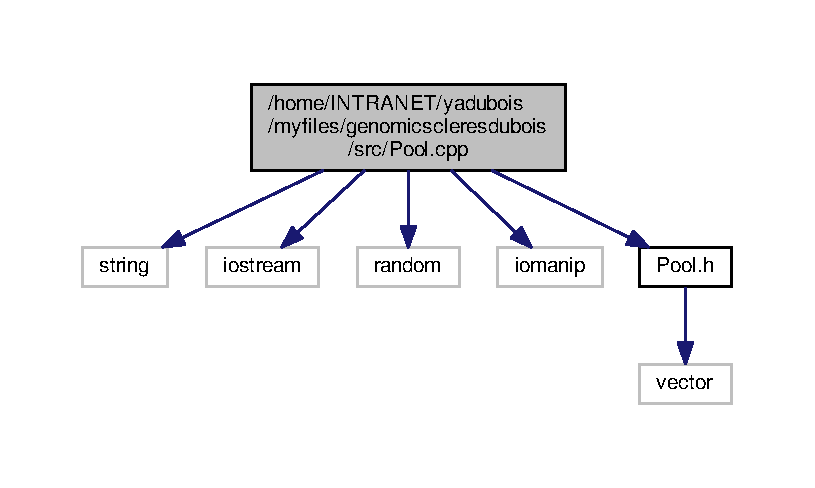
\includegraphics[width=350pt]{Pool_8cpp__incl}
\end{center}
\end{figure}


\subsection{Detailed Description}
description pool \begin{DoxyAuthor}{Author}
Yann Dubois et David C\-Leres 
\end{DoxyAuthor}
\begin{DoxyDate}{Date}
10 Novembre 2015 
\end{DoxyDate}
\begin{DoxyVersion}{Version}
1.\-0 
\end{DoxyVersion}

\hypertarget{Pool_8h}{\section{/home/\-I\-N\-T\-R\-A\-N\-E\-T/yadubois/myfiles/genomicscleresdubois/src/\-Pool.h File Reference}
\label{Pool_8h}\index{/home/\-I\-N\-T\-R\-A\-N\-E\-T/yadubois/myfiles/genomicscleresdubois/src/\-Pool.\-h@{/home/\-I\-N\-T\-R\-A\-N\-E\-T/yadubois/myfiles/genomicscleresdubois/src/\-Pool.\-h}}
}


generates a pool of alleles  


{\ttfamily \#include \char`\"{}vector\char`\"{}}\\*
Include dependency graph for Pool.\-h\-:
\nopagebreak
\begin{figure}[H]
\begin{center}
\leavevmode
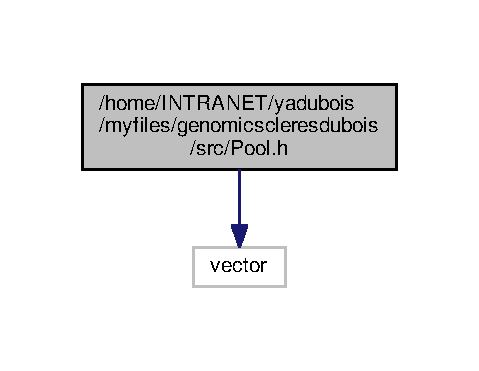
\includegraphics[width=230pt]{Pool_8h__incl}
\end{center}
\end{figure}
This graph shows which files directly or indirectly include this file\-:
\nopagebreak
\begin{figure}[H]
\begin{center}
\leavevmode
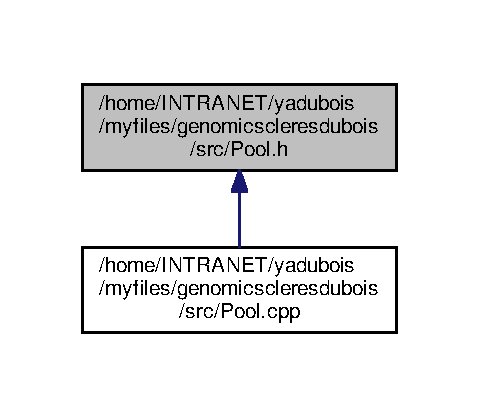
\includegraphics[width=230pt]{Pool_8h__dep__incl}
\end{center}
\end{figure}
\subsection*{Classes}
\begin{DoxyCompactItemize}
\item 
class \hyperlink{classPool}{Pool}
\begin{DoxyCompactList}\small\item\em generator class \end{DoxyCompactList}\end{DoxyCompactItemize}


\subsection{Detailed Description}
generates a pool of alleles \begin{DoxyAuthor}{Author}
Yann Dubois \& David Cleres 
\end{DoxyAuthor}
\begin{DoxyDate}{Date}
10 november 2015 
\end{DoxyDate}
\begin{DoxyVersion}{Version}
1.\-0 description 
\end{DoxyVersion}

%--- End generated contents ---

% Index
\newpage
\phantomsection
\addcontentsline{toc}{chapter}{Index}
\printindex

\end{document}
